\documentclass{beamer}

% Packages.

% Presentation metadata.
\title{Minetest - Tinctures}
\author{Frostsnow}
\date{April 13th, 2024}

\usetheme[hideothersubsections]{Hannover}
\usecolortheme{sidebartab}

\begin{document}

% Title.
\begin{frame}
  \titlepage
\end{frame}

\section{Background}
\begin{frame}{Minetest}
\begin{itemize}
	\item Voxel-based game engine
	\item Totally not a clone of that other game
	\item Designed around mods
	\item game == group of mods
\end{itemize}
\end{frame}

\begin{frame}{Tinctures}
\begin{itemize}
	\item \underline{Revelation}: text-based "MUD"
	\item Tinctures: random high-level drop
	\item Apply to item, permanent enchantment or BOOM!
	\item Could be fun in Minetest\ldots
\end{itemize}
\end{frame}

\section{Implementation}
\begin{frame}{Initial commit}
\begin{itemize}
	\item \texttt{minetest.register\_tool()}?
	\begin{itemize}
		\item Combinatorial explosion
		\item Required at load time
	\end{itemize}
	\item \texttt{minetest.override\_item()} updates server metadata, not client
	\item \small \texttt{itemstack:get\_meta():set\_tool\_capabilities(caps)} Works!
	\item Tincture data: stored in tool's \texttt{MetaData} object
	\begin{itemize}
		\item get/set string/int/float methods
		\item Hold tincture counts and metadata version
	\end{itemize}
\end{itemize}
\end{frame}

\begin{frame}{Description}
\begin{itemize}
	\item Roman numerals
	\item \texttt{description} part of \texttt{MetaData}
	\item Handles newlines
	\item \texttt{minetest.colorize()} for color
	\item 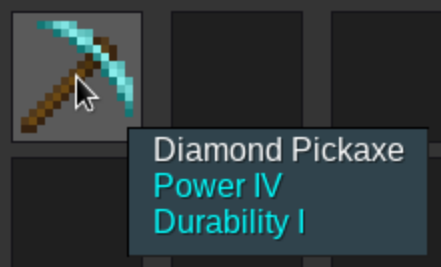
\includegraphics[scale=0.33]{description.png}
\end{itemize}
\end{frame}

\begin{frame}{Damage}
\begin{itemize}
	\item Tool capabilities \emph{damage groups}.
	\item Only \texttt{fleshy} exists.
	\item But it was an int\ldots
	\item "Carry" damage?
	\item \texttt{minetest.register\_on\_punchnode()} for digging, not LUA entities (mobs)
	\item Mobs mod overrides \texttt{on\_punch()}\ldots~also overrides wear
	\item No luck; players have to deal with truncated int damage
\end{itemize}
\end{frame}

\begin{frame}{Fortune?  Efficiency!}
\begin{itemize}
	\item "Accumulate" extra ore in tool, give when past a threshold
	\item More tinctures accumulate ore faster
	\item \texttt{minetest.register\_on\_dignode()} to implement
	\item Check for ore via \texttt{minetest.registered\_ore()}, right?
	\item Wrong!  Sand and dirt counted as ``ores''
	\item Easy hack: match against name \texttt{stone\_with\_...}
	\item \texttt{inventory:room\_for\_items()} or \texttt{minetest.add\_item()} to give extra items from drop list
	\item No idea how probablistic drops work with \texttt{get\_node\_drops()}
\end{itemize}
\end{frame}

\begin{frame}{Explosion}
\begin{itemize}
	\item Damage: \texttt{player:set\_hp()}
	\item Knockback: $\pm 15^{\circ}$ horizontally, $10-15^{\circ}$ vertically
	\begin{itemize}
		\item \texttt{player:get\_look\_horizontal()}
		\item \texttt{minetest.yaw\_to\_dir()}
		\item \texttt{vector.rotate()}
		\item \texttt{player:add\_velocity()}
	\end{itemize}
	\item Sound: \texttt{minetest.sound\_play()}, sound from Freesound
	\item Crater: \texttt{minetest.dig\_node()} from player location at \texttt{player:get\_pos()}
	\item Smoke effect:
	\begin{itemize}
		\item \texttt{minetest.add\_particlespawner()}
		\item Dig texture from node, but not node\ldots
		\item Use minified entire image\ldots
	\end{itemize}
\end{itemize}
\end{frame}

\begin{frame}{Essences}
\begin{itemize}
	\item Need to prevent tincture removal on tool breakage
	\item Can override \texttt{tool:after\_use()}, but only at initialization\ldots
	\item Enumerate all tools with \texttt{minetest.registered\_tools} table
	\item Caveat: tools must be loaded, include as \emph{dependency} of tinctures
	\item What to actually do in override?
	\item Item instantly breaks at max wear
	\item Drop "memory" of tool and tinctures, called \emph{essence}
	\item Register tool and essence recipe with \texttt{minetest.register\_craft()}
	\item Recipe is static, need \texttt{minetest.register\_on\_craft()} and \texttt{minetest.register\_craft\_predict()}
\end{itemize}
\end{frame}

\begin{frame}[fragile]{Essences (cont.)}
\begin{itemize}
	\item Handling already-tinc'd items
	\begin{itemize}
		\item Overwrite?  Dangerous\ldots
		\item Swap?  Probably okay
	\end{itemize}
	\item Handling repair
	\begin{itemize}
		\item Two worn items to one less worn item
		\item Repair two tinctured items?
		\item Apply one tincture, drop the other
	\end{itemize}
	\item Essence icon
	\begin{itemize}
		\item Use GIMP \texttt{supernova} effect, crop to quarter and mirror for symmetry
		\item Use \emph{texture modifiers} to brighten and overlay original tool on supernova
		\item Ex: \tiny\verb-inventory_image = "essence.png" .. "^[combine:32x32:8,8=" ..- \\
			\verb-tool.inventory_image .. "^[brighten"-
	\end{itemize}
\end{itemize}
\end{frame}

\begin{frame}{Tidying up}
\begin{itemize}
	\item Freesound for efficiency tinc sound effect
	\item Real icons for tinctures (remove placeholder)
	\begin{itemize}
		\item Texture modifiers as for essences
		\item Gradient Flare effect ftw
	\end{itemize}
	\item Refactor tincture application into recipe
	\item Other misc.~fix-ups\ldots
	\item Hosted on Codeberg\footnote{\texttt{https://codeberg.org/frostsnow/tinctures}}
\end{itemize}
\end{frame}

\begin{frame}{Demo}
\begin{itemize}
	\item Praise be to the demo gods!
	\item Show\ldots
	\begin{itemize}
		\item Tooltip
		\item Regular explosion
		\item 1,000 tincs explosion
	\end{itemize}
	\item The end!
\end{itemize}
\end{frame}

\end{document}
